\documentclass[conference]{IEEEtran}
\IEEEoverridecommandlockouts
% The preceding line is only needed to identify funding in the first footnote. If that is unneeded, please comment it out.
\usepackage{cite}
\usepackage{amsmath,amssymb,amsfonts}
\usepackage{algorithmic}
\usepackage{float}
\usepackage{graphicx}
\usepackage{textcomp}
\usepackage{xcolor}
\newcommand{\argmax}[1]{\underset{#1}{\operatorname{arg}\,\operatorname{max}}\;}
\newcommand{\argmin}[1]{\underset{#1}{\operatorname{arg}\,\operatorname{min}}\;}
\def\BibTeX{{\rm B\kern-.05em{\sc i\kern-.025em b}\kern-.08em
    T\kern-.1667em\lower.7ex\hbox{E}\kern-.125emX}}
\begin{document}

\title{Application of the Extended Kalman Filter in Visual-inertial Simultaneous Localization and Mapping (SLAM)}


\author{\IEEEauthorblockN{Joseph Bell}
\IEEEauthorblockA{\textit{Department of Electrical and Computer Engineering} \\
\textit{University of California, San Diego}\\
jjbell@eng.ucsd.edu}
}

\maketitle

\begin{abstract}
This paper presents an approach to solving the simultaneous localization and mapping problem through the application of the Extended Kalman filter using visual and inertial measurements. The SLAM approach was tested in three independent environments of similar setting. The results of this SLAM approach were satisfactory as they depict more accurate visual representations of the path taken by the vehicle when compared to a dead reckoning approach.
\end{abstract}

\begin{IEEEkeywords}
SLAM, EKF, Extended, Kalman Filter, visual, inertial
\end{IEEEkeywords}

\section{Introduction}

SLAM has a wide array of applications, from autonomous driving to the exploration of uncharted territories. SLAM is often considered a chicken and egg problem due to the dependencies that localization and mapping have on each other. However, in cases where neither the map nor location of the system/robot are known, localization and mapping work simultaneously to gradually refine the position of the robot/system and mapping of its environment. 

A current, real-life application of SLAM is Google's self driving car which uses a range finder to generate maps of it's environment - these maps are used in conjunction with it's previously generated maps of the world so that it can drive itself autonomously. In this case, SLAM helps Google's car navigate robustly without being thrown off by slight perturbations and new objects in the environment. The ability for robots to navigate in new environments is crucial for exploration as most of this planet (and other planets) is not habitable for humans. Robots have the ability to explore areas that are too dangerous for humans, and it is very tricky, if not impossible, for a robot to navigate in an environment that no human has been to before without the application of an algorithm like SLAM.

The goal of this paper is to detail an approach to SLAM in localization of a vehicle's trajectory through a neighborhood and mapping of features in its environment. The vehicle is equipped with an IMU and a stereo camera to gather data. This paper will first introduce the problem formulation and will follow with an explanation of the technical approach and methods used to implement this SLAM approach. The last section of this paper contains results and discussion on the performance of this SLAM approach. 


\section{Problem Formulation}


Implement visual-inertial simultaneous localization and mapping (SLAM) using the Extended Kalman Filter equations with a prediction step based on SE(3) kinematics
and an update step based on the stereo camera observation model. Perform localization and landmark mapping of a vehicle progressing throughout a neighborhood. An image of the environment captured by the stereo camera can be seen below in Figure 1. 

\begin{figure}[H]
\centerline{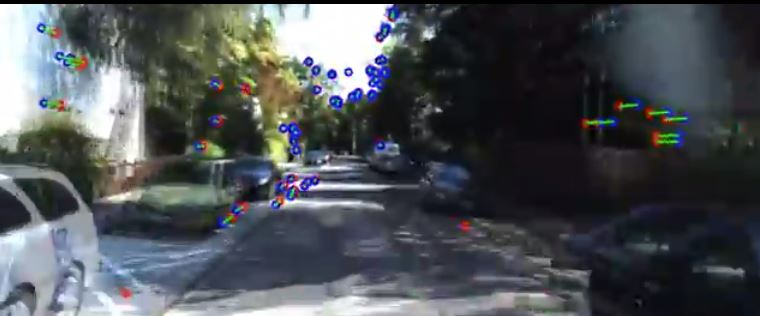
\includegraphics[width=80mm]{neighborhood.jpg}}
\caption{The neighborhood and extracted features }
\end{figure} 


\section{Technical Approach}

The total approach consists of 3 steps that will each be detailed separately. 

\subsection{Predicting the Pose}
The prediction step is responsible for estimating the pose of the vehicle in the world coordinate frame. The pose being estimated in this approach is the inverse IMU pose ($ U_{t}$), where $ U_{t} = {}_{w}{T}_{I}^{-1}$ i.e. the inverse of the transformation from the IMU to the world. The linear and angular velocity, represented by $v_{t} \in \Re^{3}$ and $\omega_{t} \in \Re^{3}$ respectively, were measured by the IMU. In combination, the estimated pose, linear velocity, and angular velocity form the motion model: 

\begin{figure}[H]
\centerline{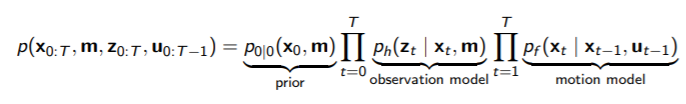
\includegraphics[width=70mm]{eqns/eq1.jpg}}
\end{figure} 


Expressing the pose as a nominal pose $\mu \in \Re^{3}$ with small perturbation $\delta \mu \in se(3)$ and solving the kinematics for the pose, the nominal pose parameters can be written as:

\begin{figure}[H]
\centerline{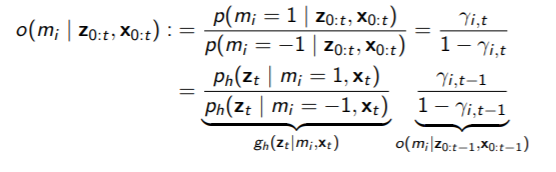
\includegraphics[width=70mm]{eqns/eq4.jpg}}
\end{figure} 

where $w_{t} \thicksim N(0,W)$ and was sampled using numpy's normal.random function.


After time discretization, the final equations for the prediction step can be written as:

\begin{figure}[H]
\centerline{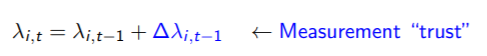
\includegraphics[width=80mm]{eqns/eq6.jpg}}
\end{figure} 

Although using the closed-form equation for the exponential map calculation in the prediction step may have been more accurate, the expm function from the scipy linear algebra library was used due to its ease of implementation and due to the fact that it provided desirable end results.

The priors for the prediction step were initialized such that:
\begin{figure}[H]\begin{figure}[H]
\centerline{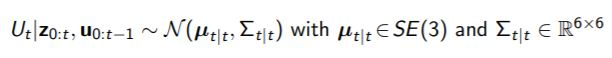
\includegraphics[width=80mm]{eqns/prior_pred.jpg}}
\end{figure} 

where $\mu_{t|t}$ was initialized as the identity matrix and each value of $\Sigma_{t|t}$ was initialized to $1E^{-6}$. 
\end{figure} 


\subsection{Mapping the Landmarks}

Data for map features was provided in the form of pixel coordinates of the feature locations at specific time stamps of video captured by the the stereo camera.
The feature in world coordinates was expressed as a nominal coordinate with $\mu_{t} \in \Re^{3}$ and $\Sigma_{t} \in \Re^{3x3}$.
Using the current pose prediction, the predicted pixel coordinate is:

\begin{figure}[H]
\centerline{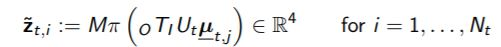
\includegraphics[width=60mm]{eqns/eq13.jpg}}
\end{figure} 

where $M := $ the calibration matrix extrinsics, ${}_{O}T_{I} (\in SE(3)) :=$ the transformation from IMU to optical frame, and $N_{t} := $ the number of time stamps.

The observation model is represented as:
\begin{figure}[H]
\centerline{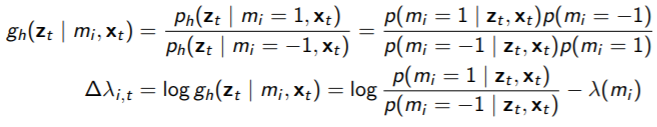
\includegraphics[width=70mm]{eqns/eq7.jpg}}
\end{figure} 

where the measurement noise of observation $i$ is $v_{t+1, i} \thicksim N(0,V) $ and was sampled using numpy's normal.random function.

The mapping step is defined as an update step, and therefore requires a Kalman Gain to be calculated. The formula for the Kalman Gain is:

\begin{figure}[H]
\centerline{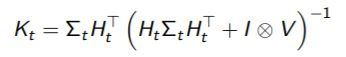
\includegraphics[width=40mm]{eqns/kg.jpg}}
\end{figure} 

where H is the jacobian of the predicated pixel values with respect to the landmark world coordinates evaluated at $\mu$:

\begin{figure}[H]
\centerline{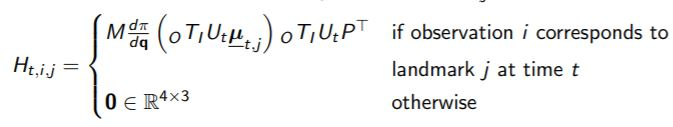
\includegraphics[width=60mm]{eqns/H.jpg}}
\end{figure} 

The final update equations for the feature mapping are as follows:

\begin{figure}[H]
\centerline{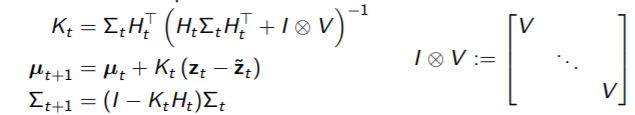
\includegraphics[width=60mm]{eqns/eq20.jpg}}
\end{figure} 

For the initialization of landmark coordinates, a list was used to keep track of which features had been seen before and which features were being seen for the first time. If a feature is being seen for the first time the $\mu$ parameter is initialized by solving for it in the pixel coordinate prediction equation introduced at the very beginning of this section. Ever value of the $\Sigma$ parameter was also initialized to $1E^{-6}$. 
\subsection{Updating the Pose}

The final step of the SLAM approach is to refine the pose using the mapped observations via an update step on the pose. The equation for the predicted pixel position can be rewritten as:

\begin{figure}[H]
\centerline{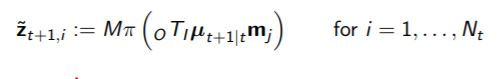
\includegraphics[width=50mm]{eqns/eq14.jpg}}
\end{figure} 

which is the same as the previous equation for predicting the pixel coordinates except the parameter being estimated this time is $\mu$ for the pose of the vehicle.

Taking the jacobian of the predicted pixel with respect to $U_{t+1}$ evaluated at $\mu_{t+t|t}$ results in:

\begin{figure}[H]
\centerline{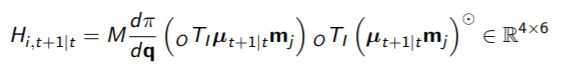
\includegraphics[width=60mm]{eqns/eq11.jpg}}
\end{figure} 

The final equations for updating the pose are as follows:

\begin{figure}[H]
\centerline{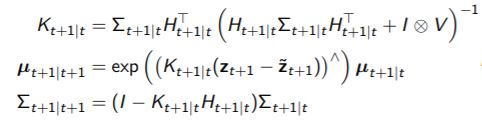
\includegraphics[width=60mm]{eqns/eq12.jpg}}
\end{figure} 



\section{Results and Discussion}

The trajectories that resulted from dead-reckoning and the application of the extended Kalman filter can be observed at the end of this section in Figures 3 through 8.

The success of the EKF approach to SLAM was determined by visually comparing the recorded video of the vehicle trajectory to the generated trajectory plots. Also, the professor had informed us that for data set 1 the vehicle ends at the starting point, for data set 2 the streets before and after turning should be parallel, and for data set 3 the vehicle took a sharp right turn toward the end and not a U-turn. Based on these facts and the output plots in Figures 3 through 8, I can clearly conclude the EKF was successful in better tracking the trajectory of the vehicle through the neighborhood.

Just as in the last project, data management was necessary for debugging purposes. The feature data was down-sampled in order to quickly observe effects on the trajectory from code changes. Once the algorithm implementation was correct with the down sampled data, noise parameters were adjusted to hone in on accurate noise distribution parameters for the full set of observations. Other than down-sampling the data by some constant factor, one other approach to down-sample the data was to limit the number of feature points based on their appearance frequency. Since the pose update works by comparing feature positions at varying poses, and every feature is not seen in every pose, if a feature is not seen that often then it is not providing much benefit to the algorithm and doesn't warrant the additional computation time - at least that's what seems intuitive.

A plot was generated, shown in Figure 2, illustrating the frequency of observations for each feature. After observing this plot, it's clear to see that the distribution of frequencies of observations among features is not even - some features are observed a vast number more than others. 

\begin{figure}[H]
\centerline{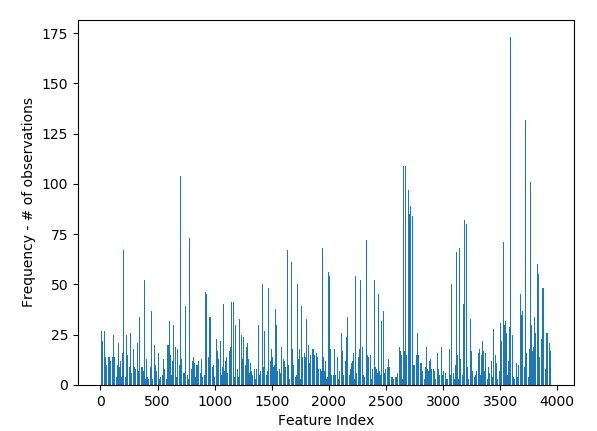
\includegraphics[width=60mm]{eqns/frequencyplot.jpg}}
\caption{Frequency of feature observations}
\end{figure} 


A threshold was set on the frequency of feature observations to only use the top 25 percent of features in regard to frequency of observation. Although it wasn't expected, the EKF was more successful when all the features were used. It's possible this threshold was too strict and even though some features were only observed a few times, they could still be providing valuable information to the pose update. If I had more time I would continue to research behavior to see if quality beats quantity in this application of the EKF.

In the figures at the end of this section, the green points are landmarks, the red line is the trajectory, the blue point is the starting point, the blue arrows show the vehicle orientation at that point, and the orange point is the ending point.

\begin{figure}[H]
\centerline{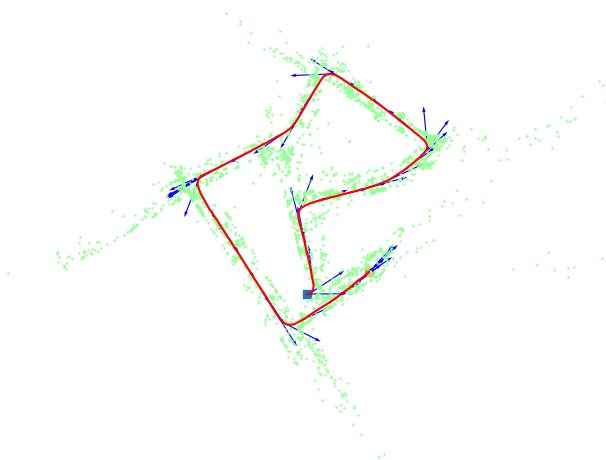
\includegraphics[width=60mm]{mapping_27.png}}
\caption{Trajectory from dead-reckoning for data set 1}
\end{figure} 
\begin{figure}[H]
\centerline{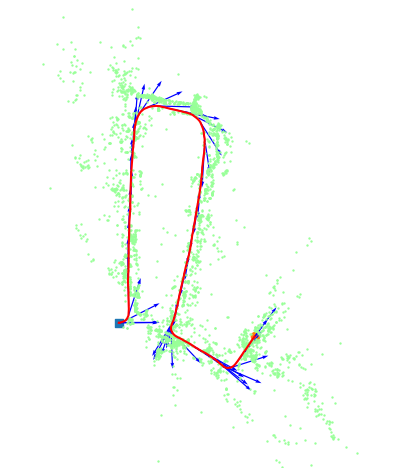
\includegraphics[width=60mm]{mapping_22.png}}
\caption{Trajectory from dead-reckoning for data set 2}
\end{figure} 
\begin{figure}[H]
\centerline{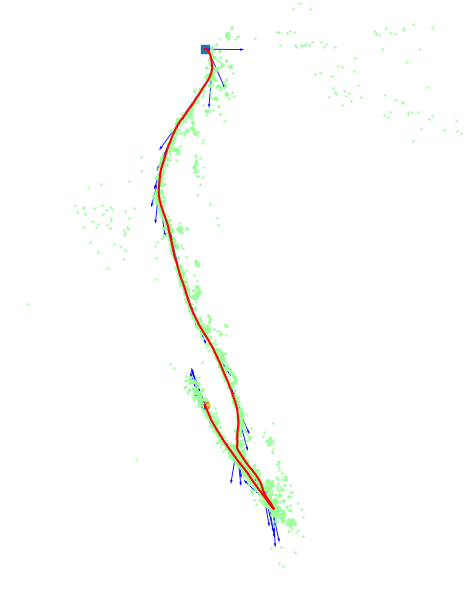
\includegraphics[width=60mm]{mapping_34.png}}
\caption{Trajectory from dead-reckoning for data set 3}
\end{figure} 

\begin{figure}[H]
\centerline{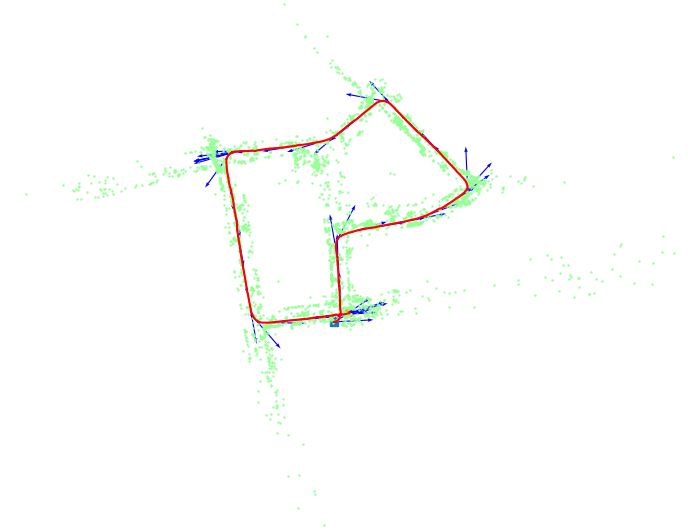
\includegraphics[width=60mm]{final27.png}}
\caption{Trajectory from EKF for data set 1}
\end{figure} 
\begin{figure}[H]
\centerline{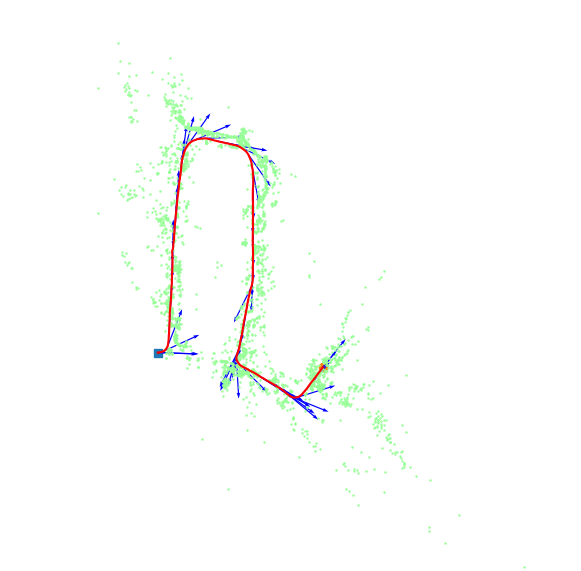
\includegraphics[width=70mm]{final22.png}}
\caption{Trajectory from EKF for data set 2}
\end{figure} 
\begin{figure}[H]
\centerline{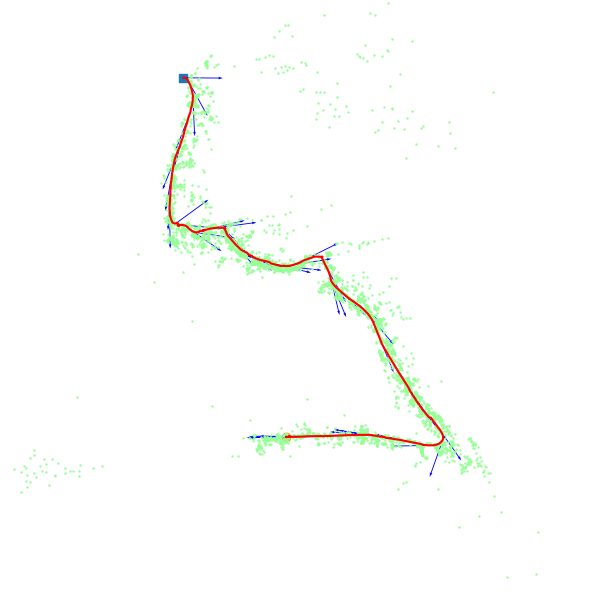
\includegraphics[width=70mm]{final34.png}}
\caption{Trajectory from EKF for data set 3}
\end{figure} 




\begin{thebibliography}{00}
\bibitem{b1} https://natanaso.github.io/ece276a
\end{thebibliography}
\end{document}
